\documentclass[a4paper,10pt]{article}
\usepackage[margin=1.0in]{geometry}

%%%%%%%%%%%%%%%%%%%%%%% Page header and setup %%%%%%%%%%%%%%%%%%%%%%%
\usepackage{fancyhdr}
\pagestyle{fancy}
\fancyhf{}
\lhead{\footnotesize Nicholas Molyneaux}
\rhead{\footnotesize 2015}

\cfoot{\thepage}

%%%%%%%%%%%%%%%%%%%%%%% Bibliography style %%%%%%%%%%%%%%%%%%%%%%%
\bibliographystyle{plain}
\usepackage{varioref}
\usepackage{natbib}

\usepackage{siunitx}
\usepackage{mathtools} % norm and absolute value

\DeclarePairedDelimiter\abs{\lvert}{\rvert}%
\DeclarePairedDelimiter\norm{\lVert}{\rVert}%

% Swap the definition of \abs* and \norm*, so that \abs
% and \norm resizes the size of the brackets, and the 
% starred version does not.

\makeatletter
\let\oldabs\abs
\def\abs{\@ifstar{\oldabs}{\oldabs*}}
%
\let\oldnorm\norm
\def\norm{\@ifstar{\oldnorm}{\oldnorm*}}
\makeatother

%%%%%%%%%%%%%%%%%%%%%%% Figure related packages %%%%%%%%%%%%%%%%%%%%%%%
\usepackage{graphicx}
\usepackage{pdfpages} % for inserting pdfs
\usepackage{epstopdf}
\usepackage[font=small,margin=1cm]{caption}
\usepackage[margin=1cm]{subcaption}
\usepackage{standalone} % inserting full standalone tex files
\usepackage{tabularx} % allows the specification of the tabular width
\newcommand{\inputTikz}[2]{%specify width for tikz images
     \scalebox{#1}{\input{#2}}  
}
\usepackage{float} % allows using of [H] for figures
\usepackage{adjustbox} % allows wide figures
%%%%%%%%%%%%%%%%%%%%%%% TIKZ related packages %%%%%%%%%%%%%%%%%%%%%%%
\usepackage{tikz}
\usepackage{pgfplots}
\usetikzlibrary{arrows}
\usepackage{xparse}
\usetikzlibrary{calc}
\usepackage{pgfplotstable}
\input{$HOME/TexConfig/tikz.tex}

%\usepackage{amssymb}
%\usepackage{amsthm}
\usepackage{amsmath}
%\usepackage{float}
%\usepackage[listofformat=subparens]{subfig}
%\usepackage{natbib}
\usepackage{url}
\usepackage[utf8]{inputenc}
\usepackage[cyr]{aeguill}
\usepackage[english]{babel}
%\usepackage{xspace}
\usepackage[T1]{fontenc}
%\usepackage{pdfpages}
%\usepackage{lscape}
%\usepackage{tocbibind}
%\usepackage{epstopdf}
%\usepackage{multirow}
%\usepackage{rotating}
%\usepackage{varioref}
%\usepackage{hyperref}
%\usepackage{cleveref}

%% Adds the subfigures to the list of figures
%\renewcommand{\thesubfigure}{\thefigure.\arabic{subfigure}}
%\captionsetup[subfigure]{labelformat=simple,labelsep=colon,
%listofformat=subsimple}
%\captionsetup{lofdepth=2}
%\makeatletter
%\renewcommand{\p@subfigure}{}
%\makeatother
%%

%% Adds a newpage before each section
%%\let\stdsection\section
%%\renewcommand\section{\newpage\stdsection}




%%%%%%%%%%%%%%%%%%%%%%%%%%%%%%%%%%%%%%%%%%%%%%%%%%%%%%%%%%%%%%%%%%%%%
%					Start of the main document
%%%%%%%%%%%%%%%%%%%%%%%%%%%%%%%%%%%%%%%%%%%%%%%%%%%%%%%%%%%%%%%%%%%%%
\begin{document}
\setlength{\parindent}{0pt}
\setlength{\parskip}{5pt plus 1pt minus 1pt}

%%%%%%%%%%%%%%%%%%%%%%% Title  %%%%%%%%%%%%%%%%%%%%%%%
\title{N-Body parallelization with MPI\\ DRAFT}
\author{Nicholas Molyneaux}
\vspace{-4cm}
\maketitle


%%%%%%%%%%%%%%%%%%%%%%% Document %%%%%%%%%%%%%%%%%%%%%%%

\section{N-Body}
The n-body simulations are relevant for many fields of science, from planet and galaxy interactions all the way down to molecular dynamics. The computational challenge comes from the fact that all bodies have some effect on all the others. The effect comes from the gravitational pull each body has on the others, the force one body of mass $m_1$ has on another of mass $m_2$ depends on the distance between each body $r$ and the gravitational constant $G$. The formula is the following:
\[\boldsymbol{\norm{F}} = G\frac{m_1m_2}{r^2}\]
where $G=\SI{6.674e-11}{Nm^{2}kg^{-2}}$. The direction of the force is given by the center of masses of the objects in the following way, where $p_1$ and $p_2$ are the positions of both masses. 
\begin{align*}
F_x &= \norm{\boldsymbol{F}}\frac{p_{2,x}-p_{1,x}}{r}\\
F_y &= \norm{\boldsymbol{F}}\frac{p_{2,y}-p_{1,y}}{r}
\end{align*}
\subsection{Complexity}
A classical brute-force approach to this problem has a complexity of $\boldsymbol{\mathcal{O}(n^2)}$, where $n$ is the number of bodies in the system. This will rapidly become unbearable, since for 1000 bodies the calculations take the order of one second on a laptop. Since this problem is time dependant, the calculations must be performed at each time step, hence the importance of having a parallel application to perform the body interactions is obvious. The copmutation of the interactions at each step is straight forward, using two loops the force on each body induced by the other bodies is calculated.\\
One well-known solution to this problem is the Barnes-Hut algorithm. This method calculates the forces acting between one body, and a group of bodies represented by the average of the group's masses and positions. With this algorithm, the complexity is reduced to $\boldsymbol{\mathcal{O}(nlogn)}$. In this case, the world (i.e. collection of bodies) is stored in a structure called ``quad-tree'', where each node stores the average of the bodie's positions and masses. At the leaves there is either a body if it fits into the quadrant, or nothing if no body is present. To calculate the interactions between all bodies, we traverse all bodies, and based on a distance criteria we either calculate the interaction with the exact body or the interaction with an ``averaged body''. 

\subsection{Computations vs communications}
For a simple brut-force approach, the computations follow $\mathcal{O}(n^2)$ at each time step. To guarantee correct results, the acceleration, velocity and position of all bodies must be updated in a synchronized manner, hence one cannot move forward in time until all forces have been calculated. Once the new positions are calculated for all bodies on each node, these updated positions must be broadcast to all other nodes so they can continue the compuations at the next time step. Therefore the communication complexity is $\mathcal{O}(n)$, since the positions of the bodies must be passed around between nodes. The ratio of computations to communications can be approximated as $\mathcal{O}(n)$ for the parallel brute-force approach.\\
For Barnes-Hut's algorithm, this ratio remains the same. The choice is made to rebuild the quad-tree from scratch at each time iteration, this makes the implementation much easier and the time taken is not significant compared to the computation time. With this in mind, the communications are the same as for the brute-force approach, since at each time step the positions and velocities of each body must be passed to all compute nodes again. Therefore the calculations are in $\mathcal{O}(nlogn)$ and the communications are $\mathcal{O}(n)$.
\subsection{Amdahl's Law}
Since the goal is the analyse the parallel aspects of the problem, the time taken to write the results to a file at each time step are not taken into account. This part is significant and limits the speedup values to very poor ones. In both cases, the initial data is stored in a file which must be read to get the initial positions and velocities.  
\paragraph{Brute-Force} For the brut force approach, since the data is stored in arrays, very little pre-processing is required. The fraction of non-parallelizable code is very low, it is only loading the data from a file. XXX PERFORM CORECT MESAURMENETS Some quick measurements give a fraction $f=0.005$ as the serial part. Hence the optimistic upper bound for the speed can be calculated and plotted. For the improved estimation, the communication fraction can be estimated to $f_{comm} = 0.015$, which takes into account the time to distribute the inital situation to the nodes. The data which must be distributed is the mass, initial velocities and positions to all nodes. Hence the new ``realistic'' speedup graph is shown below, Figure \ref{fig:th_su}. This speedup graph is still far too optimistic as it does not take into account the communication at each time step.\\

\paragraph{Quad-Tree}
For a quad-tree method, the serial part is still only reading the initial data. Since each node builds its own quad-tree, the serial part remains only reading the initial data. Hence the initial communication will be the distribution of the initial positions and velocities. The measurements which are performed for the brute-force approach are still valid, as the difference happens during the time iterations. Except that now the computation time is significantly faster, hence the fraction of serial code is larger.  With this regard, the optmistic upperbound will not be as high as previously since the computations are in $\mathcal{O}(nlogn)$ (and not $\mathcal{O}(n^2)$) , but the communications are the same. Figure \ref{fig:th_su} shows a first estimate of the speedup, based on the measurements of the serial execution time.\\

\begin{figure}[H]
\documentclass[border=2pt]{standalone}
\usepackage{pgfplots}

\begin{document}
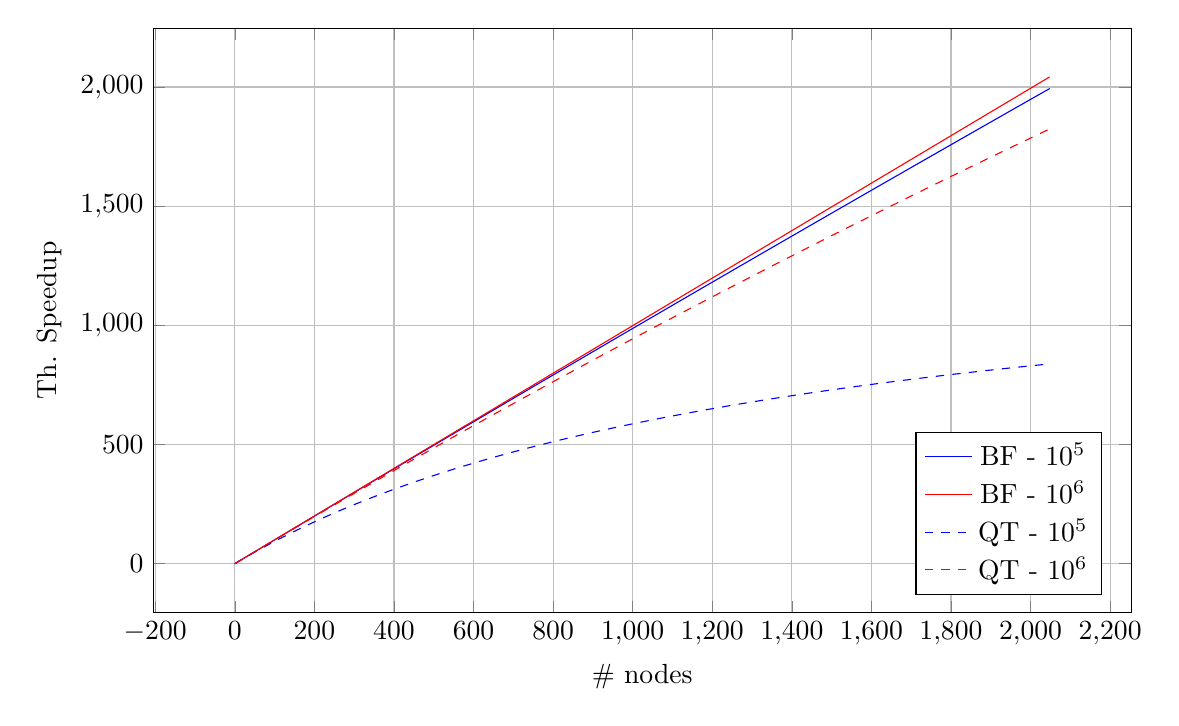
\begin{tikzpicture}
  \begin{axis}[
      xlabel= \# nodes,
      ylabel = Th. Speedup,
      ylabel style={rotate=0},
      width=14cm,
      height=9cm,
      grid=major,
      scaled x ticks = false,
      legend entries={BF - $10^5$, BF - $10^6$, QT - $10^5$, QT - $10^6$},
      legend pos = south east,
      tick label style={/pgf/number format/fixed},
    ]
    \addplot[solid,blue, domain=0:2048, samples=500] {x/(1+(x-1)*0.0000133333)};
    \addplot[solid,red, domain=0:2048, samples=500] {x/(1+(x-1)*0.00000133333)};
    \addplot[dashed,blue, domain=0:2048, samples=500] {x/(1+(x-1)*0.000705)};
    \addplot[dashed,red, domain=0:2048, samples=500] {x/(1+(x-1)*0.00006)};

\end{axis}
\end{tikzpicture}
\end{document}

\caption{Theoretical speedup chart for both the brut-force approach and the quad-tree method. These are estimations based on some simple timings on a serial implementation.}
\label{fig:th_su}
\end{figure}

%f = 0.001 hence max is very high.
%Required communicatpon: positions swapped times n_procs. gigabit eternet: 125MB/s latency: 0.125ms
%fcomm = 0.015           ftot = 0.001 hence plot theoretical best and lower best.


\section{Parallelization strategy}
The choice for MPI was justified by the need for industry and the universal aspect of the message passing interface paradigm. For the n-body problem, the messages to be passed are the mainly the updated positions of the bodies which were calculated on the other nodes. An efficient way of storing the data must be conceived to minimize the transfer times and allow the Barnes-Hut algorithm to run. As mentionned previously, two strategies are implemented. A brute-force approach and the Barnes-Hut algorithm. The strategy for the first is clear whereas for the second further work needs doing.
\subsection{Brut-Force flowgraph} With this methodology the only data which is exchanged is the updated positions. For this brut-force approach, this data must be updated at each time step, hence less data cannot be transfered. The output of the positions at each time step could be done in parallel using MPI's write methods, but at this stage this is not done. 
\begin{figure}[H]
\centering
\inputTikz{0.95}{../figures/flowchart_bf.tex}
\caption{Flowchart for the brut-force parallel implementation. Once the initial data is sent to all nodes, they update the positions of all bodies which are assigned to them, then send to all of the other nodes the updates positions. At the end of a time step, the positions are synchronized and a new time step can be calculated. The main node will write the positions to a file at each time iteration.}
\label{fig:flow_chart_bf}
\end{figure}

\subsection{Brut-Force timing diagram}
In this case, the slowest path is straightforward to estimate. The assumption that the intial distribution of the data between the nodes is done sequentially. Once the data is distributed and the first time step calculated, the idle time of each node is only the time it takes for the master node to write the data to a file. This step could also be parallelized by either using an ``MPI\_Write'', or getting each node to write a file locally and then regrouping all the data to the main node. 
\begin{figure}[H]
\centering
\inputTikz{1}{../figures/timing_bf.tex}
\caption{Timing diagram for the BF approach. The block of computations is repeated until the final time is reached. The circled characters next to the coloured boxes refer to Figure \ref{fig:flow_chart_bf}, to emphasize that they are the same steps.}
\label{fig:timing_bf}
\end{figure} 

\subsection{Quad-Tree}
The flowgraph and timing diagram will be very similar. The main differences will reside in the initialization processes which requires to build the full tree and the type and amout of data exchange between each node. 

\section{Performance}
\begin{table}
\centering
\begin{tabular}{l|cccccccccc}
\# nodes & 1 & 2 & 4 & 8 & 12 & 16 & 20 & 24 & 28 & 32\\
\hline initial broadcast [s] & $2\cdot10^{-6}$ & 0.029 & 0.041 & 0.041 & 0.047 & 0.043 & 0.053 & 0.048 & 0.031 & 0.044\\
tree building [s] & 2.37 & 2.32 & 3.05 & 3.03 & 3.04 & 3.03 & 3.03 & 2.33 & 2.72 & 2.68\\
computations [s] & 97.8 & 48.7 & 28.64 & 11.77 & 9.89 & 7.45 & 6.012 & 3.83 & 3.9 & 3.43 \\
& - & $\pm 0.56$ & $\pm 0.71$ & $\pm 0.82$ & $\pm 0.72$ & $\pm 1.05$ & $\pm 0.43$ & $\pm 0.25$ & $\pm 0.48$ & $\pm 0.50$  \\
synchronization [s] & 0.015 & 0.015 & 0.019 & 0.025 & 0.026 & 0.026 & 0.031 & 0.029 & 0.025 &0.024\\
\end{tabular}
\caption{For $10^6$ bodies, measurements of each operation on Deneb using the Barnes-Hut algorithm.}
\label{tab:qt:measure}
\end{table}

\begin{table}
\centering
\begin{tabular}{l|cccccccccc}
\# nodes & 1 & 2 & 4 & 8 & 12 & 16 & 20 & 24 & 28 & 32\\
\hline initial broadcast [s] & $1.9\cdot10^{-6}$ & 0.0036 & 0.0048 & 0.0031 & 0.0039 & 0.0036 & 0.0037 \\
tree building [s] & 0.202 & 0.201 & 0.202 & 0.205 & 0.204 & 0.203 &0.207 \\
computations [s] & 8.24 & $4.12$ & 2.06 & 1.03 &  0.68  & 0.517 &0.420 \\
& - & $\pm 0.0055$ & $\pm 0.008$ & $\pm0.07$ & $\pm 0.04$ & $\pm 0.04$ & $\pm0.04$  \\
synchronization [s] & $1.4\cdot 10^{-3}$ & 0.0017 & 0.0025 & 0.0014 & 0.0026 &  0.0036& 0.0034 \\
\end{tabular}
\caption{For $10^5$ bodies, measurements of each operation on Deneb using the Barnes-Hut algorithm.}
\label{tab:qt:measure}
\end{table}


The perormances are expecetd to be far lower than the theoretical ones calculated previously since the communication times are neglected in the actual estimations. 
\begin{figure}
\documentclass[border=2pt]{standalone}
\usepackage{pgfplots}

\begin{document}
\begin{tikzpicture}
  \begin{axis}[
      xlabel= \# nodes,
      ylabel = Speed-up,
      ylabel style={rotate=0},
      width=14cm,
      height=9cm,
      grid=major,
      scaled x ticks = false,
      legend entries={Th. - $10^5$, Rel.  - $10^5$,Th. - $10^6$, Rel.  - $10^6$},
      legend pos = south east,
      tick label style={/pgf/number format/fixed},
    ]
    \addplot[black,dashed, domain=0:48, samples=100] {(453.94)/(0.0035 + 453.94/x + 0.0015)};
    \pgfplotstableread{../results/100000_summary.csv}\dataSmall;
    \addplot[dashed,blue, thick] table[x expr=\thisrowno{0}, y expr=453/\thisrowno{2}] {\dataSmall};

    \addplot[black,solid, domain=0:48, samples=100] {(44875)/(0.035 + 44875/x + 0.025)};
    \pgfplotstableread{../results/1000000_summary.csv}\dataLarge;
    \addplot[solid, blue, thick] table[x expr=\thisrowno{0}, y expr=44875/\thisrowno{2}] {\dataLarge};

\end{axis}
\end{tikzpicture}
\end{document}

\caption{Speedup chart for the brute-force approach.}
\end{figure}

\begin{figure}
\documentclass[border=2pt]{standalone}
\usepackage{pgfplots}

\begin{document}
\begin{tikzpicture}
  \begin{axis}[
      xlabel= \# nodes,
      ylabel = Speed-up,
      ylabel style={rotate=0},
      width=14cm,
      height=9cm,
      grid=major,
      scaled x ticks = false,
      legend entries={Th. - $10^5$, Rel.  - $10^5$,Th. - $10^6$, Rel.  - $10^6$},
      legend pos = south east,
      tick label style={/pgf/number format/fixed},
    ]
    \addplot[black, dashed, domain=0:32, samples=100] {(0.2+8.24)/(0.0038+0.2+8.24/x+0.003)};
    \pgfplotstableread{../results/100000_summary.csv}\dataSmall;
    \addplot[solid,blue,dashed, thick] table[x expr=\thisrowno{0}, y expr=8.48/\thisrowno{1}] {\dataSmall};

    \addplot[black, solid, domain=0:48, samples=100] {(2.7+97.8)/(0.045+2.7+100/x+0.03)};
    \pgfplotstableread{../results/1000000_summary.csv}\dataLarge;
    \addplot[solid,blue, thick] table[x expr=\thisrowno{0}, y expr=100.03/\thisrowno{1}] {\dataLarge};

\end{axis}
\end{tikzpicture}
\end{document}

\caption{Speedup chart for the quad-tree approach.}
\end{figure}

%%%%%%%%%%%%%%%%%%%%% bibliography %%%%%%%%%%%%%%%%%%%%%
\nocite{*}
\bibliography{../references}
%%%%%%%%%%%%%%%%%%%%% End document %%%%%%%%%%%%%%%%%%%%%
\end{document}
